\subsection{Singulärwertzerlegung}
\label{SVD}
\begin{equation*}
    \underbrace{A}_{\mathbb{R}^{m\times n}} = \underbrace{U}_{\mathbb{R}^{m\times m}} \overbrace{\Sigma}^{\mathbb{R}^{m\times n}} \underbrace{V^T}_{\mathbb{R}^{n\times n}}
\end{equation*}

\begin{itemize}
    \item \(U\) und \(V\) sind orthogonale/unitäre Matrizen
    \item \(U\) enthält die normierten Eigenvektoren von \(AA^T\); kann als eine Basis für den Spaltenraum von \(A\) betrachtet werden
    \item \(V\) enthält die normierten Eigenvektoren von \(A^TA\); kann als eine Basis für den Zeilenraum von \(A\) betrachtet werden
    \item \(\Sigma\) ist eine Diagonalmatrix mit den Singulärwerten \(\sigma_1 \geq \sigma_2 \geq \hdots \geq 0\) (sortiert) auf der Hauptdiagonalen. Die Singulärwerte sind die Wurzeln der Eigenwerte von \(A^TA\) und \(AA^T\) (\(\sigma_i = \sqrt{\lambda_i}\), Rest \(=0\)).    \item Die Singulärwerte in \(\Sigma\) geben die Stärke der Korrelation zwischen den Spalten und Zeilen von A an. Die größten Singulärwerte in \(\Sigma\) geben die wichtigsten Merkmale von A an, während die kleinsten Singulärwerte in \(\Sigma\) die Rauschkomponenten von A darstellen.
\end{itemize}


\begin{figure}[ht]
    \centering
    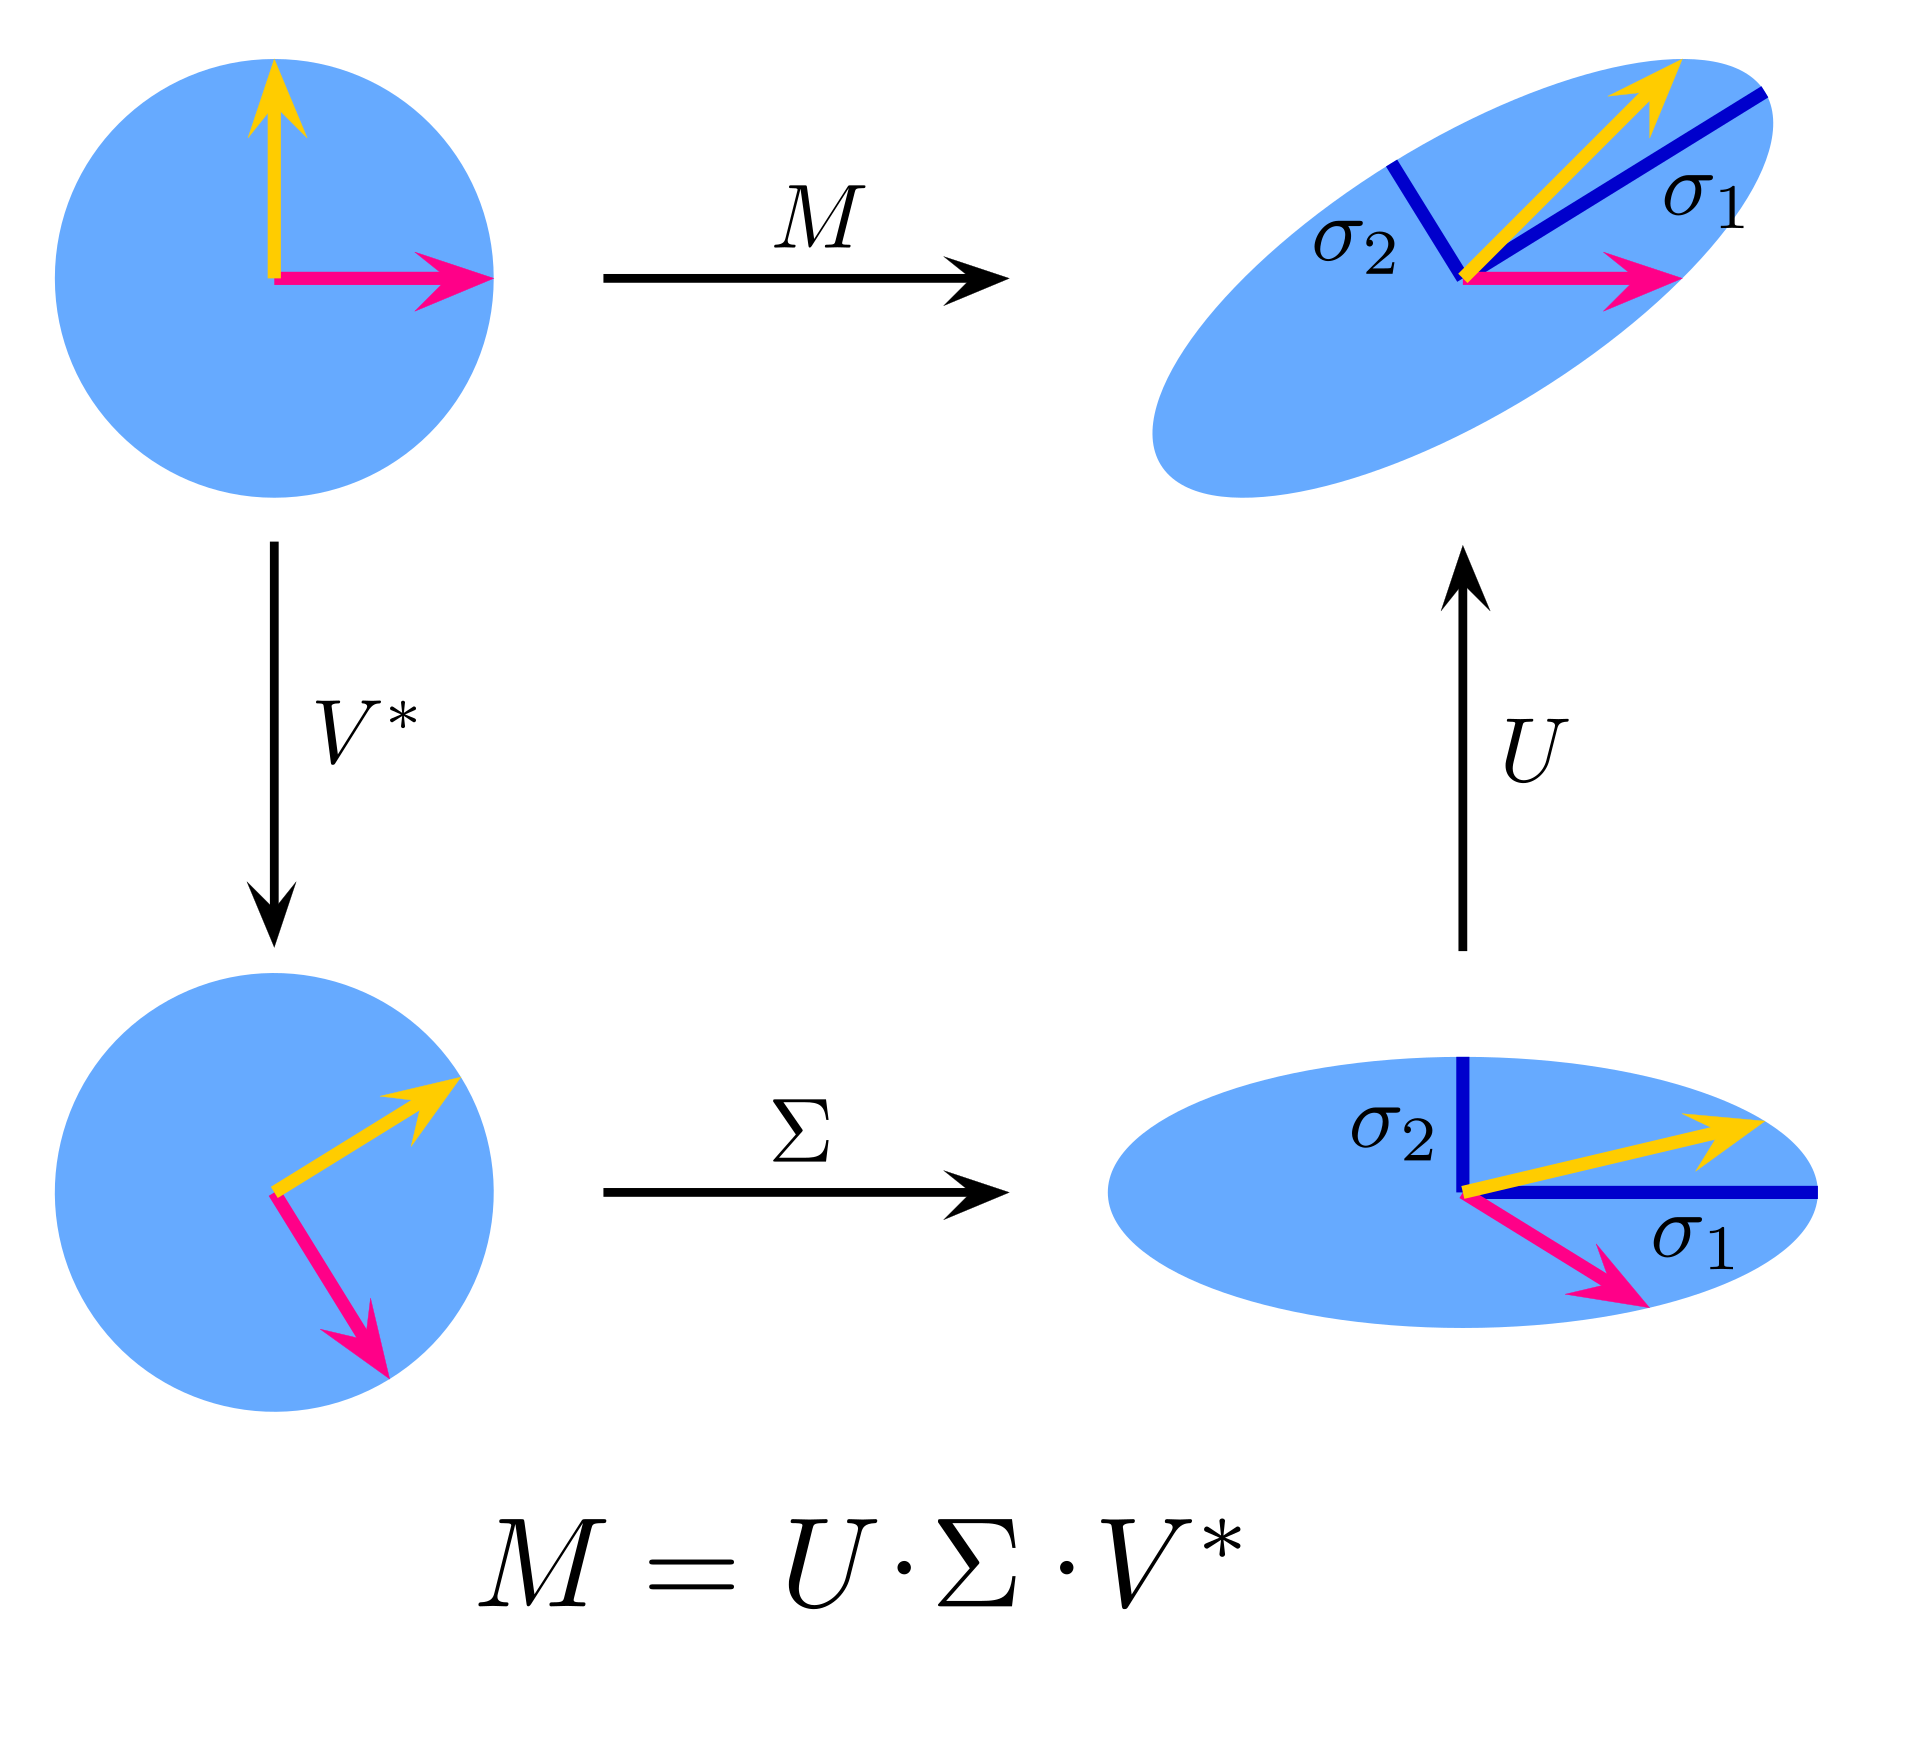
\includegraphics[width=0.5\textwidth]{lineareAlgebra/1920px-Singular-Value-Decomposition.svg.png}
    \caption*{Singulärwertzerlegung }
    \label{fig:svd}
\end{figure}

\subsubsection{Einfaches Berechnungsverfahren (über Eigenvektoren)}
\begin{enumerate}
    \item \(AA^T\) und \(A^TA\) bestimmen
    \item Für \glqq kleinere\dq Matrix aus 1) Eigenwerte \(\lambda_i\) bestimmen (char. Polynom)
    \item \(\Sigma\) mit \(diag(\sigma_1 \geq \sigma_2 \geq \hdots \geq \sigma_n)\) aufstellen; Singulärwerte \(\sigma_i = \sqrt{\lambda_i}\) auf Hauptdiagonalen; Rest \(=0\)
    \item \(U\) aufstellen: normierte Eigenvektoren für \(AA^T\) für alle \(\lambda_i\) bestimmen
    \item \(V\) aufstellen: normierte Eigenvektoren für \(A^TA\) für alle \(\lambda_i\) bestimmen; \(V^T\) bilden
\end{enumerate}



\subsubsection{Alternatives Berechnungsverfahren}

\begin{table}[H]
  \centering
  \begin{tabularx}{\textwidth}{X|l}
    %%%%%%%%%%%%%%%%%%%%%%%%%%%%%%%
    % 1. Form prüfen
    %%%%%%%%%%%%%%%%%%%%%%%%%%%%%%%
    \makecell[l]{\textbf{1. Form prüfen:} ist \(A\) \glqq hochkant\grqq? \\
        \(\rightarrow\) sonst aufwendiger zu lösen\\
        Umstellen zu \(A^T\) ist möglich, da\\
        \((A^T)^T = A\); d.h. \(A^T = V\Sigma^T U^T\)
    }
        &        
    \(A = \begin{pmatrix}       
        1 & 0 \\
        2 & 2 \\
        0 & 1
    \end{pmatrix}\)\\\\

    %%%%%%%%%%%%%%%%%%%%%%%%%%%%%%%
    % 2. Eigenwerte bestimmen
    %%%%%%%%%%%%%%%%%%%%%%%%%%%%%%%
    \makecell[l]{\textbf{2. Eigenwerte von \(A^T A\) bestimmen} \\
        Eigenwerte (\(\geq 0\)) über \textit{Nullstellen char.}\\ \textit{Polynom} bestimmen,
        absteigend sortieren!
    }
        &
    \makecell[l]{            
        \(A^TA = \begin{pmatrix}       
            5 & 4 \\
            4 & 5
        \end{pmatrix}\) \\
        \(p_A(\lambda) = \det (A^T A - \lambda I) \overset{!}{=} 0\)\\
        \((5-\lambda)^2-16=0\)\\
        \(\lambda_1 = 9, \lambda_2 = 1\)
    }\\\\

    %%%%%%%%%%%%%%%%%%%%%%%%%%%%%%%
    % 3. Sigma aufstellen
    %%%%%%%%%%%%%%%%%%%%%%%%%%%%%%%
    \makecell[l]{\textbf{3. \(\Sigma\) aufstellen} \\
        Diagonalmatrix mit \(\sigma_i=\sqrt[]{\lambda_i}\), Rest \(=0\)
    }
        &
    \makecell[l]{            
        \(\Sigma = \begin{pmatrix}       
            3 & 0 \\
            0 & 1 \\
            0 & 0
        \end{pmatrix}\)
    }\\\\

    %%%%%%%%%%%%%%%%%%%%%%%%%%%%%%%
    % 4. Spaltenvektoren für V ermitteln
    %%%%%%%%%%%%%%%%%%%%%%%%%%%%%%%
    \makecell[l]{\textbf{4. Spaltenvektoren für \(V\) ermitteln} \\
        Eigenvektoren zu \(\lambda\) aus 2. bestimmen,\\
        normieren und in Matrix \(V\) eintragen\\
        Für SVD: \(V^T\) bilden
    }
        &
    \makecell[l]{       
        \underline{für \(\lambda_1 = 9\):}\\     
        \(
            \left( 
            \begin{array}{cc|c}
                5 - 9 &  4 & 0\\
                4 & 5-9 & 0
            \end{array}
            \right)\Leftrightarrow 
        \)\\
        \(
            \left( 
            \begin{array}{cc|c}
                1 &  -1 & 0\\
                0 & 0 & 0
            \end{array}
            \right)\Rightarrow v_1^* = \begin{pmatrix}       
                1 \\
                1
            \end{pmatrix}
        \)\\
        \(v_1=\frac{v_1^*}{||v_1^*||} = \frac{1}{\sqrt{2}}\begin{pmatrix}
            1 \\
            1
        \end{pmatrix}\)\\\\
        \underline{für \(\lambda_2 = 1\):}\\ 
        \(\hdots\)\\
        \(v_2=\frac{v_2^*}{||v_2^*||} = \frac{1}{\sqrt{2}}\begin{pmatrix}
            -1 \\
            1
        \end{pmatrix}\)\\\\
        \(V = \frac{1}{\sqrt{2}}\begin{pmatrix}
            1 & -1 \\
            1 & 1
        \end{pmatrix}\)
    }\\\\

    %%%%%%%%%%%%%%%%%%%%%%%%%%%%%%%
    % 5. U aufstellen
    %%%%%%%%%%%%%%%%%%%%%%%%%%%%%%%
    \makecell[l]{\textbf{5. \(U\) aufstellen} \\
        a) für vorhandene Singulärwerte:\\ \hspace*{1.5em}\(u_i = \frac{1}{\sigma_i}Av_i\)\\
        b) sonst: \(u_i\) so finden, dass \(u_i\) ONB sind\\
            \hspace*{1.5em}\(\rightarrow\) Kreuzprodukt (\(\mathbb{R}^3\))\\
            \hspace*{1.5em}\(\rightarrow\) Gram-Schmidt
    }
        &
    \makecell[l]{            
        \(u_1 = \frac{1}{3\sqrt{2}}\begin{pmatrix}
            1\\
            4\\
            1
        \end{pmatrix}\),
        \(u_2 = \frac{1}{\sqrt{2}}\begin{pmatrix}
            -1\\
            0\\
            1
        \end{pmatrix}\)\\
        b) \(u_3=u_1\times u_2 = \frac{1}{6}\begin{pmatrix}
            4\\
            -2\\
            4
        \end{pmatrix}\)\\
    }\\\\
    \end{tabularx}
\end{table}
